%
% $RCSfile: user_interface.tex,v $
%
% Copyright (c) 2002-2007. Christian Heller. All rights reserved.
%
% Permission is granted to copy, distribute and/or modify this document
% under the terms of the GNU Free Documentation License, Version 1.1 or
% any later version published by the Free Software Foundation; with no
% Invariant Sections, with no Front-Cover Texts and with no Back-Cover
% Texts. A copy of the license is included in the section entitled
% "GNU Free Documentation License".
%
% http://www.cybop.net
% - Cybernetics Oriented Programming -
%
% Version: $Revision: 1.2 $ $Date: 2007-08-01 13:59:01 $ $Author: christian $
% Authors: Christian Heller <christian.heller@tuxtax.de>
%

\section{User Interface}
\label{user_interface_heading}
\index{User Interface}

A \emph{User Interface} (UI) provides functionality by which a user can
communicate with a software system.

%
% $RCSfile: textual_user_interface.tex,v $
%
% Copyright (c) 2002-2007. Christian Heller. All rights reserved.
%
% Permission is granted to copy, distribute and/or modify this document
% under the terms of the GNU Free Documentation License, Version 1.1 or
% any later version published by the Free Software Foundation; with no
% Invariant Sections, with no Front-Cover Texts and with no Back-Cover
% Texts. A copy of the license is included in the section entitled
% "GNU Free Documentation License".
%
% http://www.cybop.net
% - Cybernetics Oriented Programming -
%
% Version: $Revision: 1.1 $ $Date: 2007-07-17 20:02:36 $ $Author: christian $
% Authors: Christian Heller <christian.heller@tuxtax.de>
%

\subsection{Textual User Interface}
\label{textual_user_interface_heading}
\index{Textual User Interface}

\emph{Textual User Interface} (TUI) is a synonym for character-based UI.
Historically, the TUI (besides the simple command line) was the first kind of
UI for computers. It mostly offers a menu with a list of possible choices that
can be activated via the pressing of a special button on the keyboard. Figure
\ref{textual_user_interface_figure} illustrates a typical, menu-based TUI.

\begin{figure}[ht]
    \begin{center}
%        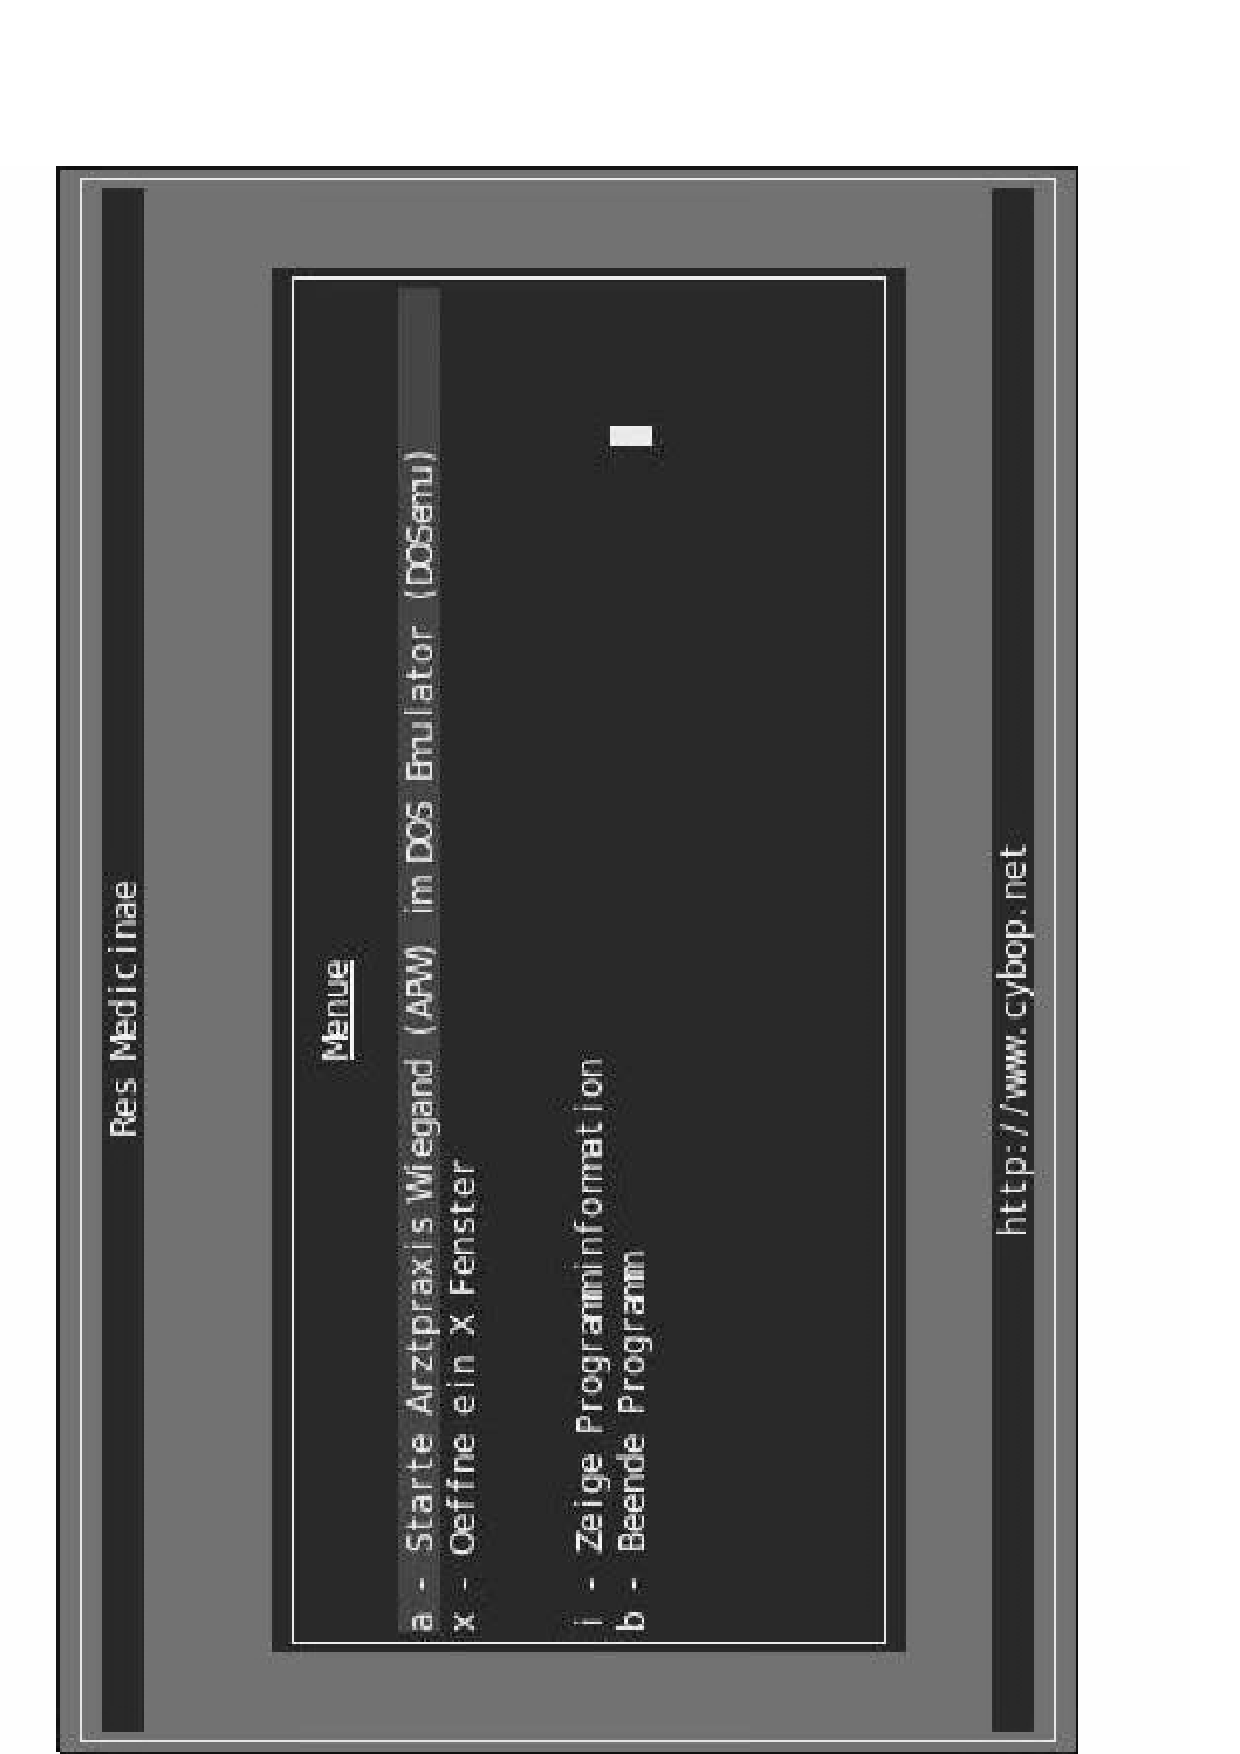
\includegraphics[scale=0.3,angle=-90]{graphics/textual_user_interface.pdf}
        \caption{Textual User Interface}
        \label{textual_user_interface_figure}
    \end{center}
\end{figure}

\subsubsection{Position Property}

\emph{required}

name=\texttt{'position'}\\
abstraction=\texttt{'integer'}\\
model=\texttt{x, y, z coordinates}

This property specifies the TUI element's origin.

\subsubsection{Size Property}

\emph{required}

name=\texttt{'size'}\\
abstraction=\texttt{'integer'}\\
model=\texttt{x, y, z extensions}

This property specifies the TUI element's extension.

\subsubsection{Background Property}

\emph{required}

name=\texttt{'background'}\\
abstraction=\texttt{'character'}\\
model=\texttt{'black' \vline\ 'red' \vline\ 'green' \vline\ 'yellow' \vline\ 'blue' \vline\ 'magenta' \vline\ 'cobalt' \vline\ 'white'}

This property specifies the background colour of the TUI.

\subsubsection{Foreground Property}

\emph{required}

name=\texttt{'foreground'}\\
abstraction=\texttt{'character'}\\
model=\texttt{'black' \vline\ 'red' \vline\ 'green' \vline\ 'yellow' \vline\ 'blue' \vline\ 'magenta' \vline\ 'cobalt' \vline\ 'white'}

This property specifies the foreground colour of the TUI.

\subsubsection{Border Property}

\emph{optional}

name=\texttt{'border'}\\
abstraction=\texttt{'character'}\\
model=\texttt{'line' \vline\ 'round\_line' \vline\ 'double\_line'}

This property specifies the kind of border of the TUI.

\subsubsection{Hidden Property}

\emph{optional}

name=\texttt{'hidden'}\\
abstraction=\texttt{'boolean'}\\
model=\texttt{'true' \vline\ 'false'}

This property specifies whether or not to hide the TUI element.

\subsubsection{Inverse Property}

\emph{optional}

name=\texttt{'inverse'}\\
abstraction=\texttt{'boolean'}\\
model=\texttt{'true' \vline\ 'false'}

This property specifies whether or not to display the TUI element in inverse
colours.

\subsubsection{Blink Property}

\emph{optional}

name=\texttt{'blink'}\\
abstraction=\texttt{'boolean'}\\
model=\texttt{'true' \vline\ 'false'}

This property specifies whether or not the TUI element should blink.

\subsubsection{Underline Property}

\emph{optional}

name=\texttt{'underline'}\\
abstraction=\texttt{'boolean'}\\
model=\texttt{'true' \vline\ 'false'}

This property specifies whether or not to underline the TUI element's text.

\subsubsection{Bold Property}

\emph{optional}

name=\texttt{'bold'}\\
abstraction=\texttt{'boolean'}\\
model=\texttt{'true' \vline\ 'false'}

This property specifies whether or not to display the TUI element's text in
bold font.

\subsubsection{Focus Property}

\emph{optional}, only if TUI element should be able to react to button press events

name=\texttt{'focus'}\\
abstraction=\texttt{'knowledge' \vline\ 'encapsulated'}\\
model=\texttt{logic knowledge model}

This property points to the TUI element (knowledge model) having focus. It is
important to find out which TUI element a key press event relates to. The focus
of a number of part elements should always be held by their corresponding
whole (compound) element.

\subsubsection{Previous Property}

\emph{optional}, only if TUI element should have a predecessor that may own the focus

name=\texttt{'previous'}\\
abstraction=\texttt{'knowledge' \vline\ 'encapsulated'}\\
model=\texttt{logic knowledge model}

This property points to the previous TUI element (knowledge model) owning focus.

\subsubsection{Next Property}

\emph{optional}, only if TUI element should have a successor that may own the focus

name=\texttt{'next'}\\
abstraction=\texttt{'knowledge' \vline\ 'encapsulated'}\\
model=\texttt{logic knowledge model}

This property points to the next TUI element (knowledge model) receiving focus.

\subsubsection{Enter Property}

\emph{optional}, only if TUI element should react to button press event;
a prerequisition is that the TUI element's \emph{focus} property value is \emph{true}

name=\texttt{'enter'}\\
abstraction=\texttt{'knowledge' \vline\ 'encapsulated'}\\
model=\texttt{logic knowledge model}

This property specifies the logic knowledge model to be executed if the
\emph{Enter} button is pressed while the TUI element has focus.

\subsubsection{Escape Property}

\emph{optional}, only if TUI element should react to button press event;
a prerequisition is that the TUI element's \emph{focus} property value is \emph{true}

name=\texttt{'escape'}\\
abstraction=\texttt{'knowledge' \vline\ 'encapsulated'}\\
model=\texttt{logic knowledge model}

This property specifies the logic knowledge model to be executed if the
\emph{Esc} button is pressed while the TUI element has focus.

\subsubsection{Arrow Up Property}

\emph{optional}, only if TUI element should react to button press event;
a prerequisition is that the TUI element's \emph{focus} property value is \emph{true}

name=\texttt{'arrow\_up'}\\
abstraction=\texttt{'knowledge' \vline\ 'encapsulated'}\\
model=\texttt{logic knowledge model}

This property specifies the logic knowledge model to be executed if the
\emph{arrow-up} button is pressed while the TUI element has focus.

\subsubsection{Arrow Down Property}

\emph{optional}, only if TUI element should react to button press event;
a prerequisition is that the TUI element's \emph{focus} property value is \emph{true}

name=\texttt{'arrow\_down'}\\
abstraction=\texttt{'knowledge' \vline\ 'encapsulated'}\\
model=\texttt{logic knowledge model}

This property specifies the logic knowledge model to be executed if the
\emph{arrow-down} button is pressed while the TUI element has focus.

\subsubsection{Arrow Left Property}

\emph{optional}, only if TUI element should react to button press event;
a prerequisition is that the TUI element's \emph{focus} property value is \emph{true}

name=\texttt{'arrow\_left'}\\
abstraction=\texttt{'knowledge' \vline\ 'encapsulated'}\\
model=\texttt{logic knowledge model}

This property specifies the logic knowledge model to be executed if the
\emph{arrow-left} button is pressed while the TUI element has focus.

\subsubsection{Arrow Right Property}

\emph{optional}, only if TUI element should react to button press event;
a prerequisition is that the TUI element's \emph{focus} property value is \emph{true}

name=\texttt{'arrow\_right'}\\
abstraction=\texttt{'knowledge' \vline\ 'encapsulated'}\\
model=\texttt{logic knowledge model}

This property specifies the logic knowledge model to be executed if the
\emph{arrow-right} button is pressed while the TUI element has focus.

%
% $RCSfile: graphical_user_interface.tex,v $
%
% Copyright (c) 2002-2007. Christian Heller. All rights reserved.
%
% Permission is granted to copy, distribute and/or modify this document
% under the terms of the GNU Free Documentation License, Version 1.1 or
% any later version published by the Free Software Foundation; with no
% Invariant Sections, with no Front-Cover Texts and with no Back-Cover
% Texts. A copy of the license is included in the section entitled
% "GNU Free Documentation License".
%
% http://www.cybop.net
% - Cybernetics Oriented Programming -
%
% Version: $Revision: 1.1 $ $Date: 2007-07-17 20:02:36 $ $Author: christian $
% Authors: Christian Heller <christian.heller@tuxtax.de>
%

\subsection{Graphical User Interface}
\label{graphical_user_interface_heading}
\index{Graphical User Interface}

A \emph{Graphical User Interface} (GUI) is mostly based on so-called graphical
\emph{Windows} which may overlap, or be ordered side-by-side on a screen.
Figure \ref{graphical_user_interface_figure} illustrates a typical GUI.

\begin{figure}[ht]
    \begin{center}
%        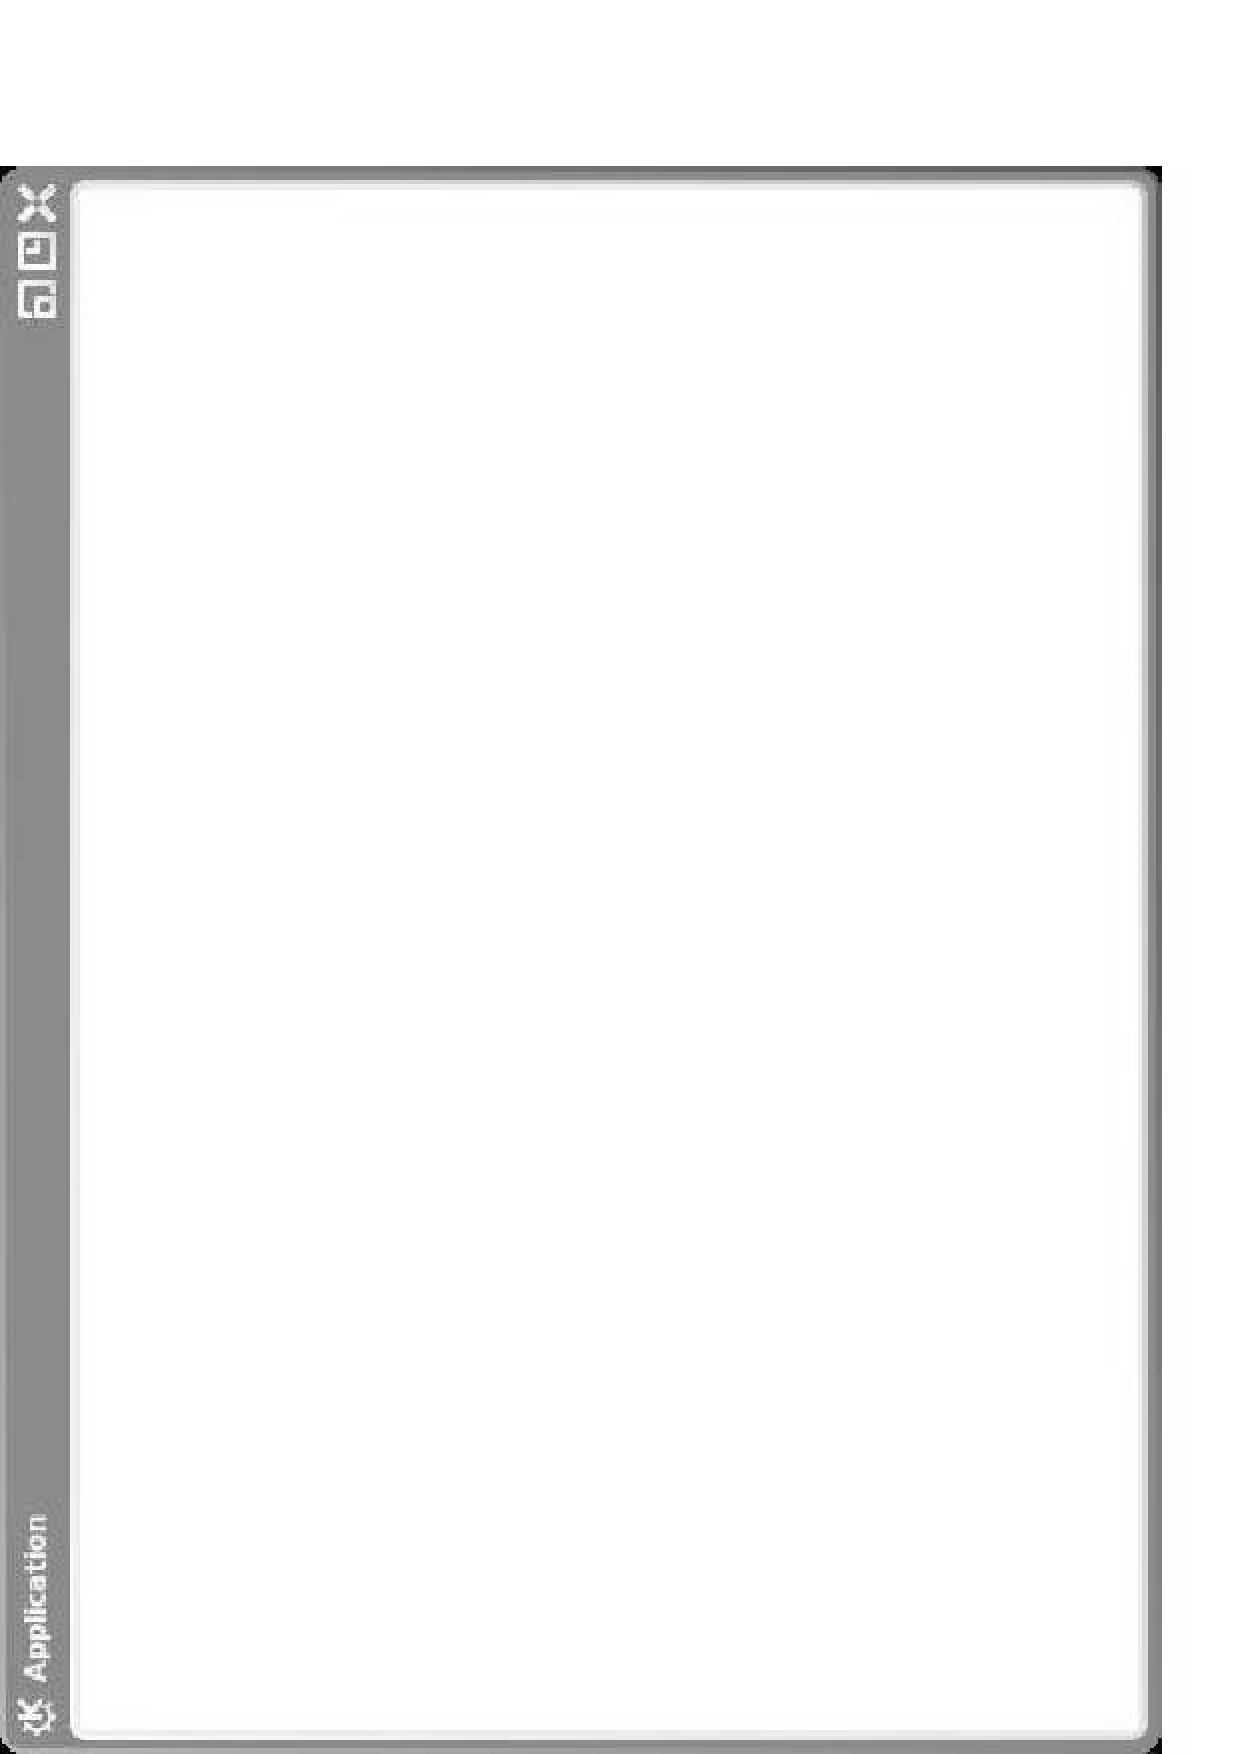
\includegraphics[scale=0.3,angle=-90]{graphics/graphical_user_interface.pdf}
        \caption{Graphical User Interface}
        \label{graphical_user_interface_figure}
    \end{center}
\end{figure}

\subsubsection{Shape Property}

\emph{required}

name=\texttt{'shape'}\\
abstraction=\texttt{'character'}\\
model=\texttt{'rectangle' \vline\ 'circle' \vline\ 'polygon'}

This property specifies the geometrical shape of the GUI.

\subsubsection{Layout Property}

\emph{required}

name=\texttt{'layout'}\\
abstraction=\texttt{'character'}\\
model=\texttt{'root' \vline\ 'coordinates' \vline\ 'compass'}

This property specifies the kind of layout of the GUI.

\subsubsection{Cell Property}

\emph{optional}, only if \emph{layout} property is \emph{compass}

name=\texttt{'cell'}\\
abstraction=\texttt{'character'}\\
model=\texttt{'north' \vline\ 'south' \vline\ 'west' \vline\ 'east' \vline\ 'centre'}

This property specifies the cell ordering, if \emph{compass} layout is used.

\subsubsection{Position Property}

\emph{required}

name=\texttt{'position'}\\
abstraction=\texttt{'integer'}\\
model=\texttt{x, y, z coordinates}

This property specifies the GUI element's origin.

\subsubsection{Size Property}

\emph{required}

name=\texttt{'size'}\\
abstraction=\texttt{'integer'}\\
model=\texttt{x, y, z extensions}

This property specifies the GUI element's extension.

\subsubsection{Background Property}

\emph{optional}

name=\texttt{'background'}\\
abstraction=\texttt{'character'}\\
model=\texttt{'black' \vline\ 'red' \vline\ 'green' \vline\ 'yellow' \vline\ 'blue' \vline\ 'magenta' \vline\ 'cobalt' \vline\ 'white'}

This property specifies the background colour of the GUI.

\subsubsection{Foreground Property}

\emph{optional}

name=\texttt{'foreground'}\\
abstraction=\texttt{'character'}\\
model=\texttt{'black' \vline\ 'red' \vline\ 'green' \vline\ 'yellow' \vline\ 'blue' \vline\ 'magenta' \vline\ 'cobalt' \vline\ 'white'}

This property specifies the foreground colour of the GUI.

\subsubsection{Title Property}

\emph{optional}, only if \emph{layout} property is \emph{root}

name=\texttt{'title'}\\
abstraction=\texttt{'character'}\\
model=\texttt{window title}

This property specifies the GUI element's (window's) title.

\subsubsection{Icon Property}

\emph{optional}, only if \emph{layout} property is \emph{root}

name=\texttt{'icon'}\\
abstraction=\texttt{'bmp' \vline\ 'jpeg' \vline\ 'png' \vline\ 'gif' \vline\ etc.}\\
model=\texttt{graphic file}

This property specifies the GUI element's (window's) icon.

\subsubsection{Expose Property}

\emph{optional}, only if GUI element should react to expose event

name=\texttt{'expose'}\\
abstraction=\texttt{'knowledge' \vline\ 'encapsulated'}\\
model=\texttt{logic knowledge model}

This property specifies the logic knowledge model to be executed if the GUI
element is exposed, for example shown again after having been hidden before.

\subsubsection{Mouse Over Property}

\emph{optional}, only if GUI element should react to mouse event

name=\texttt{'mouse\_over'}\\
abstraction=\texttt{'knowledge' \vline\ 'encapsulated'}\\
model=\texttt{logic knowledge model}

This property specifies the logic knowledge model to be executed if the mouse
is moved over the GUI element.

\subsubsection{Mouse Wheel Property}

\emph{optional}, only if GUI element should react to mouse event

name=\texttt{'mouse\_wheel'}\\
abstraction=\texttt{'knowledge' \vline\ 'encapsulated'}\\
model=\texttt{logic knowledge model}

This property specifies the logic knowledge model to be executed if the mouse
wheel is scrolled while the mouse pointer is over the GUI element.

\subsubsection{Left Press Property}

\emph{optional}, only if GUI element should react to mouse event

name=\texttt{'left\_press'}\\
abstraction=\texttt{'knowledge' \vline\ 'encapsulated'}\\
model=\texttt{logic knowledge model}

This property specifies the logic knowledge model to be executed if the left
mouse button is pressed.

\subsubsection{Left Release Property}

\emph{optional}, only if GUI element should react to mouse event

name=\texttt{'left\_release'}\\
abstraction=\texttt{'knowledge' \vline\ 'encapsulated'}\\
model=\texttt{logic knowledge model}

This property specifies the logic knowledge model to be executed if the left
mouse button is released.

\subsubsection{Left Click Property}

\emph{optional}, only if GUI element should react to mouse event

name=\texttt{'left\_click'}\\
abstraction=\texttt{'knowledge' \vline\ 'encapsulated'}\\
model=\texttt{logic knowledge model}

This property specifies the logic knowledge model to be executed if the left
mouse button is clicked. A mouse click is the combination of a mouse press- and
release event.

%
% $RCSfile: web_user_interface.tex,v $
%
% Copyright (c) 2002-2007. Christian Heller. All rights reserved.
%
% Permission is granted to copy, distribute and/or modify this document
% under the terms of the GNU Free Documentation License, Version 1.1 or
% any later version published by the Free Software Foundation; with no
% Invariant Sections, with no Front-Cover Texts and with no Back-Cover
% Texts. A copy of the license is included in the section entitled
% "GNU Free Documentation License".
%
% http://www.cybop.net
% - Cybernetics Oriented Programming -
%
% Version: $Revision: 1.2 $ $Date: 2007-08-01 13:59:01 $ $Author: christian $
% Authors: Christian Heller <christian.heller@tuxtax.de>
%

\subsection{Web User Interface}
\label{web_user_interface_heading}
\index{Web User Interface}

A \emph{Web User Interface} (WUI) is what is commonly also known as
\emph{Hypertext Markup Language} (HTML) file. HTML files get interpreted by a
\emph{Web Browser} which renders the graphical and textual information to
display these as HTML page. Figure \ref{web_user_interface_figure} shows an
example WUI.

\begin{figure}[ht]
    \begin{center}
        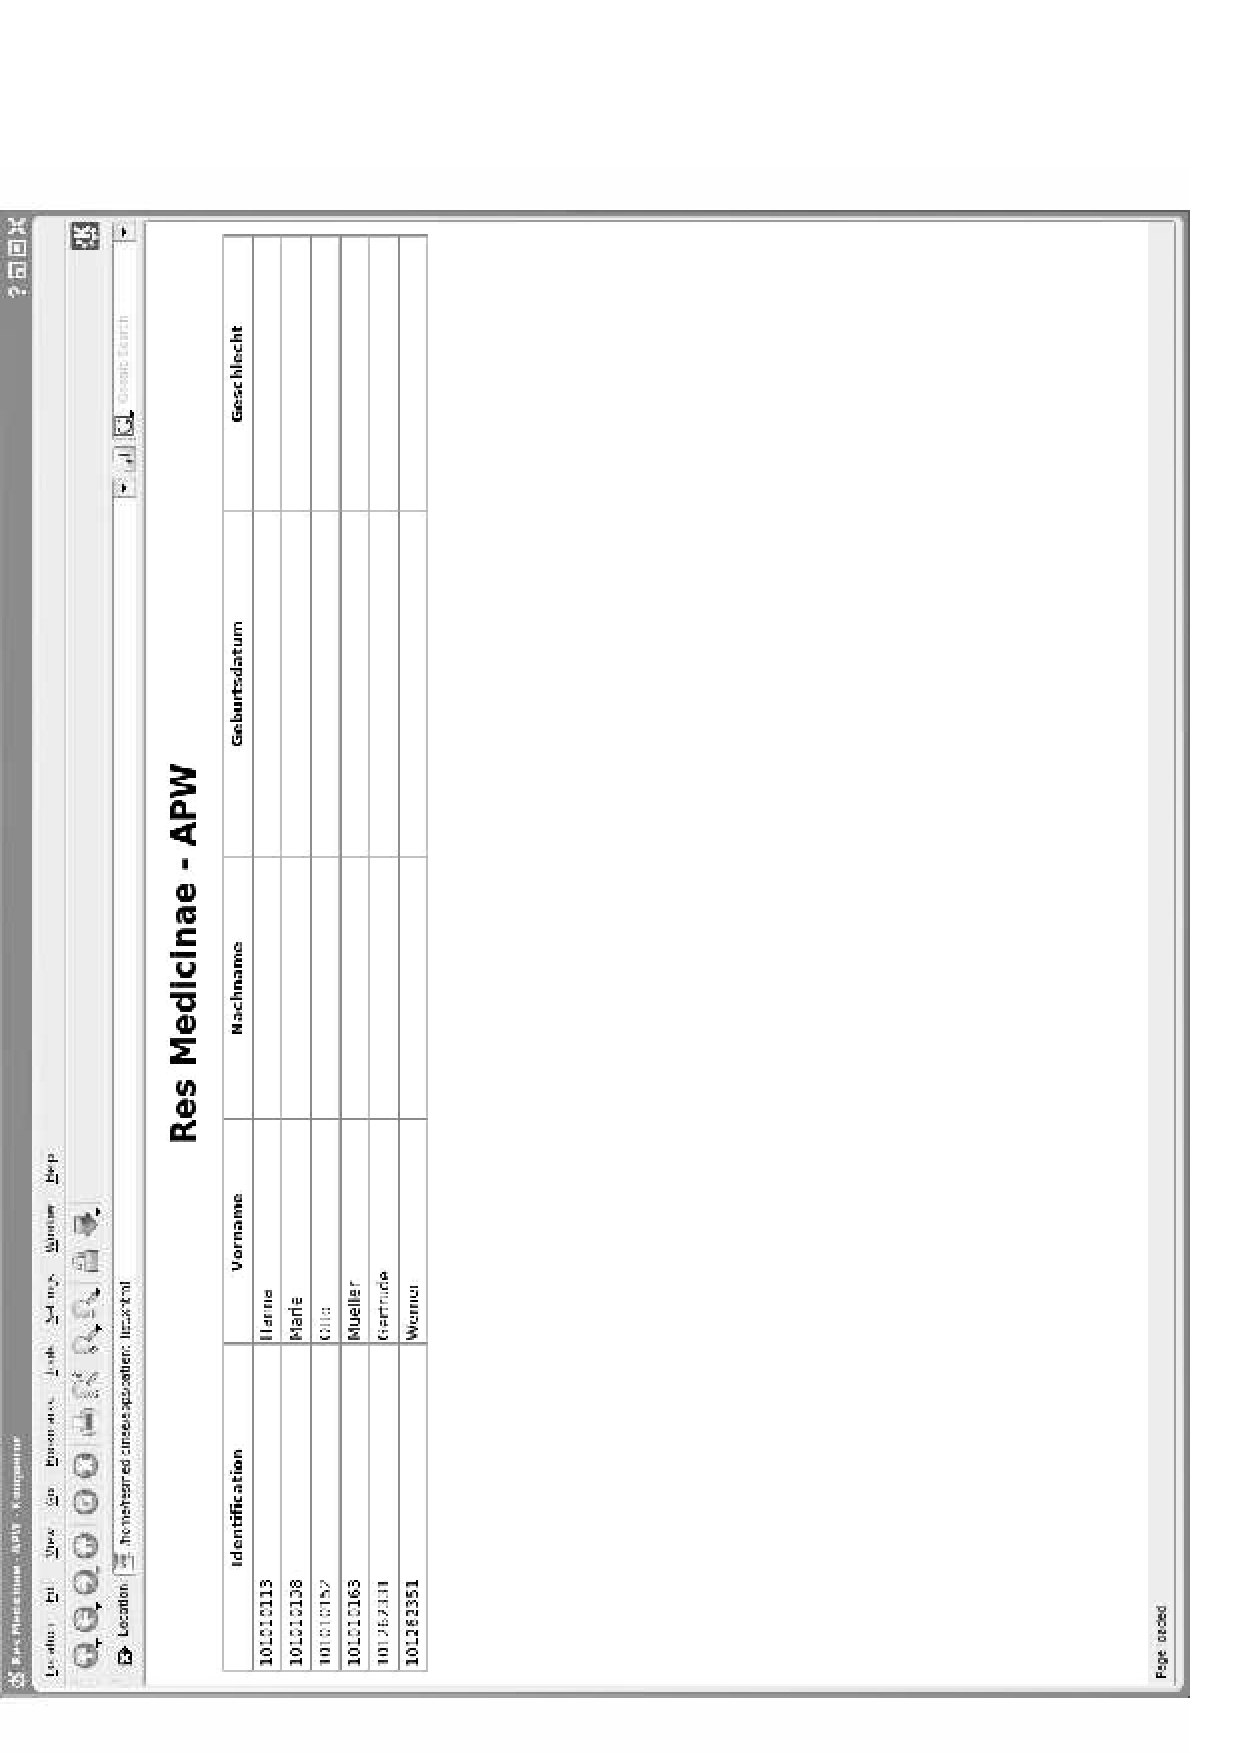
\includegraphics[scale=0.3,angle=-90]{graphics/web_user_interface.pdf}
        \caption{Web User Interface}
        \label{web_user_interface_figure}
    \end{center}
\end{figure}

\subsubsection{Example}

\begin{scriptsize}
    \begin{verbatim}
<part name="address_table" channel="file" abstraction="compound" model="wui/table.cybol">
    <property name="tag" channel="inline" abstraction="character" model="table"/>
    <property name="width" channel="inline" abstraction="character" model="100%"/>
    <property name="cellspacing" channel="inline" abstraction="integer" model="5"/>
    <property name="cellpadding" channel="inline" abstraction="integer" model="2"/>
    <property name="border" channel="inline" abstraction="boolean" model="false"/>
</part>
    \end{verbatim}
\end{scriptsize}

\subsubsection{Tag Property}

This property specifies the HTML tag to associate with the knowledge model.

\emph{required}

name=\texttt{'tag'}\\
abstraction=\texttt{'character'}\\
model=\texttt{'html' \vline\ 'head' \vline\ 'meta' \vline\ 'body' \vline\ 'table' \vline\ 'tr' \vline\ etc.}

\subsubsection{Xmlns Property}

This property specifies the XML namespace for the HTML page to be generated
from the WUI.

\emph{optional}, only for \emph{html} tag

name=\texttt{'xmlns'}\\
abstraction=\texttt{'character'}\\
model=\texttt{'http://www.w3.org/1999/xhtml'}

\subsubsection{HTTP-Equiv Property}

This property specifies the content type for the HTML page to be generated from
the WUI.

\emph{optional}, only for \emph{meta} tag

name=\texttt{'http-equiv'}\\
abstraction=\texttt{'character'}\\
model=\texttt{'content-type'}

\subsubsection{Name Property}

This property specifies the name of a meta data entry for the HTML page to be
generated from the WUI.

\emph{optional}, only for \emph{meta} tag

name=\texttt{'name'}\\
abstraction=\texttt{'character'}\\
model=\texttt{'author'}

\subsubsection{Content Property}

This property specifies the content of a meta data entry for the HTML page to
be generated from the WUI.

\emph{optional}, only for \emph{meta} tag

name=\texttt{'content'}\\
abstraction=\texttt{'character'}\\
model=\texttt{'Generated by CYBOI'}

\subsubsection{Align Property}

This property specifies the alignment of the HTML heading.

\emph{optional}, only for \emph{h1..6} tag

name=\texttt{'align'}\\
abstraction=\texttt{'character'}\\
model=\texttt{'left' \vline\ 'right' \vline\ 'center'}

\subsubsection{Width Property}

This property specifies the width of the HTML table.

\emph{optional}, only for \emph{table} tag

name=\texttt{'width'}\\
abstraction=\texttt{'character'}\\
model=\texttt{table width}

\subsubsection{Cellspacing Property}

This property specifies the spacing between the cells of the HTML table.

\emph{optional}, only for \emph{table} tag

name=\texttt{'cellspacing'}\\
abstraction=\texttt{'character'}\\
model=\texttt{space between cells in pixels}

\subsubsection{Cellpadding Property}

This property specifies the space between an HTML table cell's border and its
content.

\emph{optional}, only for \emph{table} tag

name=\texttt{'cellpadding'}\\
abstraction=\texttt{'character'}\\
model=\texttt{space between cell border and content}

\subsubsection{Border Property}

This property specifies the width of the HTML table's border.

\emph{optional}, only for \emph{table} tag

name=\texttt{'border'}\\
abstraction=\texttt{'character'}\\
model=\texttt{table border width}

\subsubsection{HRef Property}

This property specifies the reference (link) to be invoked when activating the
HTML element.

\emph{optional}, only for \emph{a} tag

name=\texttt{'href'}\\
abstraction=\texttt{'character'}\\
model=\texttt{an HTML reference}

